
%\documentclass[preprint,a4paper]{elsarticle}
\documentclass[final,3p,times,twocolumn]{elsarticle}
%\documentclass[review,3p,number,times]{elsarticle}
\usepackage{lineno}


%
%%%%%%%%%%%%%%%%%%%%%%%%%%%%%%%%%%%%%%%%%
%  Default packages
%%%%%%%%%%%%%%%%%%%%%%%%%%%%%%%%%%%%%%%%%
%
\usepackage{graphicx}
\usepackage{subfig}
\usepackage{calorimeter}
\usepackage{mathptmx}
\usepackage{helvet}
\usepackage{amsmath}
\usepackage{color}
\usepackage{units}
\usepackage{url}
\usepackage{xspace}
\usepackage{booktabs}
\usepackage{multirow}
\usepackage{wrapfig}
\usepackage{upgreek}
\usepackage{threeparttable}
%\usepackage[varg]{txfonts}
\usepackage{slashed}

%\hyphenation{CLIC-Pfo-Selec-tor}
%
%%%%%%%%%%%%%%%%%%%%%%%%%%%%%%%%%%%%%%%%%
% This is where the document really begins
%%%%%%%%%%%%%%%%%%%%%%%%%%%%%%%%%%%%%%%%%
%
\journal{Nucl. Instr. and Meth. A}

\begin{document}
  \begin{frontmatter}
%%     \begin{flushright} 
%%       CU-HEP-12/12 \\
%%       August 2012
%%     \end{flushright}   
    
    % Title of the paper
    \title{Design of an Electromagnetic Calorimeter for use at a future\\ e$^{+}$e$^{-}$ Linear Collider}
    
    % Author(s) of the paper
    \author[a]{J. S. Marshall\corref{cor1}}
    \ead{marshall@hep.phy.cam.ac.uk}
    
    % Affiliations
    \address[a]{Cavendish Laboratory, University of Cambridge, Cambridge, United Kingdom}
     \cortext[cor1]{Corresponding author}

%~~~~~~~~~~~~~~~~~~~~~~~~~~~~~~~~~~~~~~~~~~~~~~~~~~~~~~~~
% 1) Abstract
%~~~~~~~~~~~~~~~~~~~~~~~~~~~~~~~~~~~~~~~~~~~~~~~~~~~~~~~~
    \begin{abstract}
Lorem ipsum dolor sit amet, consectetuer adipiscing elit, sed diam nonummy nibh euismod tincidunt ut laoreet dolore magna aliquam erat volutpat. Ut wisi enim ad minim veniam, quis
nostrud exerci tation ullamcorper suscipit lobortis nisl ut aliquip ex ea commodo consequat. Duis autem vel eum iriure dolor in hendrerit in vulputate velit esse molestie consequat,
vel illum dolore eu feugiat nulla facilisis at vero eros et accumsan et iusto odio dignissim qui blandit praesent luptatum zzril delenit augue duis dolore te feugait nulla facilisi.
Nam liber tempor cum soluta nobis eleifend option congue nihil imperdiet doming id quod mazim placerat facer possim assum. Typi non habent claritatem insitam; est usus legentis in
iis qui facit eorum claritatem. Investigationes demonstraverunt lectores legere me lius quod ii legunt saepius. Claritas est etiam processus dynamicus, qui sequitur mutationem
consuetudium lectorum. Mirum est notare quam littera gothica, quam nunc putamus parum claram, anteposuerit litterarum formas humanitatis per seacula quarta decima et quinta
decima. Eodem modo typi, qui nunc nobis videntur parum clari, fiant sollemnes in futurum.
    \end{abstract}

    \begin{keyword}
	Particle flow calorimetry, ECAL, Linear Collider, CLIC
	%% keywords here, in the form: keyword \sep keyword
	%% MSC codes here, in the form: \MSC code \sep code
	%% or \MSC[2008] code \sep code (2000 is the default)
    \end{keyword}
  \end{frontmatter}
  
\linenumbers 

  %%%%%%%%%%%%%%%%%%%%%%%%%%%%%%%%%%%%%%%%%
  % Main part
  %%%%%%%%%%%%%%%%%%%%%%%%%%%%%%%%%%%%%%%%%

%~~~~~~~~~~~~~~~~~~~~~~~~~~~~~~~~~~~~~~~~~~~~~~~~~~~~~~~~
% 2) Introduction
%~~~~~~~~~~~~~~~~~~~~~~~~~~~~~~~~~~~~~~~~~~~~~~~~~~~~~~~~

\section{Introduction}
Lorem ipsum dolor sit amet, consectetuer adipiscing elit, sed diam nonummy nibh euismod tincidunt ut laoreet dolore magna aliquam erat volutpat. Ut wisi enim ad minim veniam, quis
nostrud exerci tation ullamcorper suscipit lobortis nisl ut aliquip ex ea commodo consequat. Duis autem vel eum iriure dolor in hendrerit in vulputate velit esse molestie consequat,
vel illum dolore eu feugiat nulla facilisis at vero eros et accumsan et iusto odio dignissim qui blandit praesent luptatum zzril delenit augue duis dolore te feugait nulla facilisi.
Nam liber tempor cum soluta nobis eleifend option congue nihil imperdiet doming id quod mazim placerat facer possim assum. Typi non habent claritatem insitam; est usus legentis in
iis qui facit eorum claritatem. Investigationes demonstraverunt lectores legere me lius quod ii legunt saepius. Claritas est etiam processus dynamicus, qui sequitur mutationem
consuetudium lectorum. Mirum est notare quam littera gothica, quam nunc putamus parum claram, anteposuerit litterarum formas humanitatis per seacula quarta decima et quinta
decima. Eodem modo typi, qui nunc nobis videntur parum clari, fiant sollemnes in futurum.

\begin{figure}[!h]
  \begin{center}
     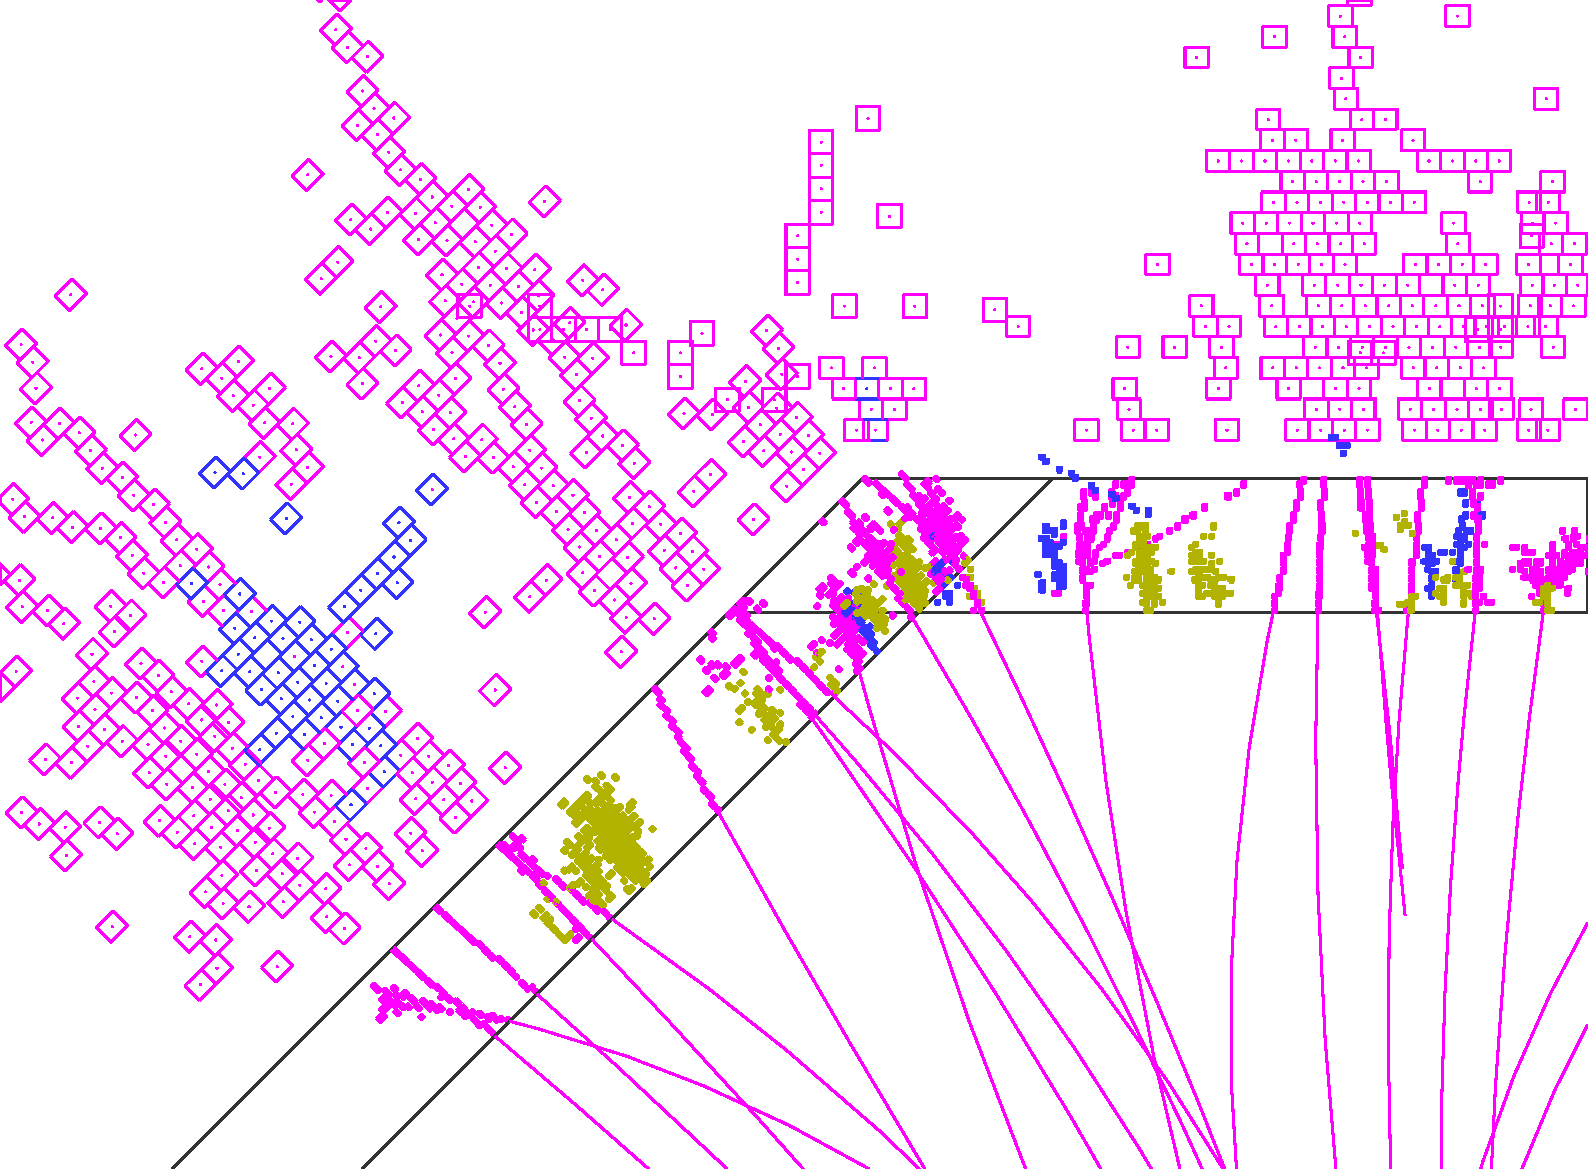
\includegraphics[width=0.45\textwidth]{EventECAL.pdf}
     \caption{\label{}}
  \end{center}
\end{figure}

%~~~~~~~~~~~~~~~~~~~~~~~~~~~~~~~~~~~~~~~~~~~~~~~~~~~~~~~~
% 3) Implementation
%~~~~~~~~~~~~~~~~~~~~~~~~~~~~~~~~~~~~~~~~~~~~~~~~~~~~~~~~

\section{Implementation}

\subsection{Simulation}

The simulation of detector model response to various physics events was performed using MOKKA.  MOKKA uses Geant4 and the geometry information for a given detector model to produce detailed simulations of detector response for various ILC detector concepts.  The flexibility in MOKKA allows various detector parameters to be modified and so optimisation studies can be performed.  In this study the optimisation was performed with respect to the ILD detector model.  

\subsection{Reconstruction}

The reconstruction of physics events was performed using the MARLIN reconstruction framework, which allows for modular implementation of various c++ programs each tasked with one aspect of the reconstruction.  While several programs are used in the full reconstruction it is important to highlight firstly to the pattern recognition implementation of particle flow calorimetry, which is done using PandoraPFA, and secondly the digitisation of calorimeter hits, implemented in the ILDCaloDigi processor.  

\begin{figure}[!h]
  \begin{center}
     \includegraphics[width=0.35\textwidth]{3_Implementation/500GeVJets.png}
     \caption{Typical topologies 250GeV jets simulated in the ILD detector model.  \label{2-jets}}
  \end{center}
\end{figure}

\subsubsection{PandoraPFA}

The PandoraPFA software package implements the pattern recognition side of particle flow calorimetry.  It is essential that calorimeter hits are correctly assigned to charged particle tracks to avoid double counting of energy in the particle flow paradigm.  This can be extremely challenging given the complex topologies associated to particle showers at high energies such as those shown in figure \ref{2-jets}.

Due to the varied nature of detector models being simulated in these studies it is necessary to have reusable and flexible software that is isolated from the detector model.  This is achieved using the Pandora Software Development Kit (PandoraSDK), which is an independent framework for applying sophisticated topological algorithms designed to perform the association of calorimeter hits to charged particle tracks.  The algorithm logic applied in PandoraSDK is independent of detector model.

\subsubsection{ILDCaloDigi}

The ILDCaloDigi processor is designed to perform the digitisation of calorimeter hits for the ILD detector model.  Digitisation of calorimeter hits is the process by which the energy deposits in the absorber (non-active) region of a calorimeter cell is estimated using the measured value of the energy deposited in the active region of the cell.  Accurate energy estimators for calorimeter cells is crucial for estimating detector performance and so calibration at this stage is essential for all simulations.  

A number of realistic effects can be simulated using the ILDCaloDigi processor, the full details of which can be found here.  For these studies electrical noise and a limited electronics read out range was simulated and the effect of timing cuts was analysed in detail.

\subsection{Calibration}

To ensure reliability in the conclusions drawn from these optimisation studies, it was necessary to calibrate the response of each detector model considered.  This occurred in three stages, the full details of which can be found here.  

Initially, the detector response to minimum ionising particles (MIPs) was determined by looking at the detector response to muons.  This set the MIP scale in both the digitiser and inside PandoraPFA, which is needed as a reference energy unit for applying thresholds and cuts.  

Secondly, the digitisation stage of the reconstruction was tuned for events of photons and long lived neutral kaons for events that were contained within the ECAL and HCAL respectively.  This tuning was an iterative procedure where constants in the digitisation processor, ILDCaloDigi, were varied and simulations repeated until the sum of calorimeter hit energies matched the Monte-Carlo energy of the photons and long lived neutral kaons being simulated.

Finally, the electromagnetic and hadronic energy scales within PandoraPFA must be correctly set.  This is done by independently scaling the energy of particle flow objects (PFOs), the output reconstructed particles from PandoraPFA, for PFOs originating from electromagnetic and hadronic showers separately.  This is again done in an iterative procedure involving changing the inputs to PandoraPFA and repeating simulations until the PFO energy matches the Monte-Carlo energy for the photons (electromagnetic showers) and long lived neutral kaons (hadronic showers) being simulated.  

\subsection{Parameterising Detector Performance}

The primary figure of merit used in these optimisation studies is the jet energy resolution, as extensively described in (Pandora paper chapter 5).  The jets used in these studies are from the decay of off-shell mass Z bosons decaying at rest into a pair of light quarks (u,d,s).  Typically, such decays form mono-energetic jets back to back as can be seen in figure \ref{2-jets}.  

Detector performance, in the particle flow paradigm, is a combination of intrinsic energy resolution and pattern recognition.  It is possible to isolate the magnitude of these two contributions to the jet energy resolution by cheating the pattern reconstruction using the Monte Carlo (MC) information, as shown in figure \ref{2-Decomp}.  Analysis of this information extends understanding of the behaviour of a detector model and will be beneficial for detector model comparisons.

A reconstruction where the pattern recognition is fully cheated provides the intrinsic energy resolution contribution to the jet energy resolution.  The quadrature difference between the default reconstruction jet energy resolution, which uses no MC information, and the fully cheated reconstruction jet energy resolution provides the confusion contribution to the jet energy resolution.  This confusion term arises due to the misidentification of the origin of some energy deposits in the detector. 

By only cheating certain aspects of the reconstruction, it is possible to decompose the confusion into terms related to the misidentification of energy deposits from certain classes of particles such as photons or neutral hadrons.  Figure \ref{2-Conf} shows a typical example of this decomposition where the photon and neutral hadron confusions have been isolated.  The other confusion is the quadrature difference between the total confusion and the sum of the photon and neutral hadron confusions.  

\begin{figure}[!h]
  \begin{center}
     \includegraphics[width=0.49\textwidth]{3_Implementation/DetailedPlot.pdf}
     \caption{Jet energy resolution as a function of jet energy for the ILD detector model.  The jet energy resolution has been decomposed into the intrinsic energy resolution and the confusion terms.  \label{2-Decomp}}
  \end{center}
    \begin{center}
     \includegraphics[width=0.49\textwidth]{3_Implementation/Confusion.pdf}
     \caption{Confusion decomposed into various terms as a function of jet energy.  Simulation was performed using the ILD detector model.  \label{2-Conf}}
  \end{center}
\end{figure}

%~~~~~~~~~~~~~~~~~~~~~~~~~~~~~~~~~~~~~~~~~~~~~~~~~~~~~~~~
% 4) Basic Detector Performance
%~~~~~~~~~~~~~~~~~~~~~~~~~~~~~~~~~~~~~~~~~~~~~~~~~~~~~~~~

\section{Default Detector Performance}
\label{Sec4}

In these studies the reference detector model will be the ILD detector model.  In this model the ECal consists of a 30 layer, silicon-tungsten ECal with a square cell size of $5\times5\text{mm}^2$ containing $\sim24$ radiation lengths ($X_0$) and $\sim1$ nuclear interaction length ($\lambda_I$).  The HCal consists of a 48 layer, scintillator-steel HCal with a square cell size of $30\times30\text{mm}^2$ containing $\sim50X_0$ and $\sim6\lambda_I$. 

In order to have confidence in the conclusions drawn from detector model comparisons, a number of parameters used in the reconstruction should be specified.  Both the timing cut placed on the simulation and the hadronic energy truncation applied to digitised HCal cells in PandoraPFA have a large impact on the detector performance.  The details of their dependancy of detector performance is described in sections \ref{TC} and \ref{HET}.

For these studies the default jet energy resolutions are shown in table \ref{Default}.

\begin{table}[h!]
\centering
\begin{tabular}{| p{1.5cm} | p{1cm} | p{1.5cm} | p{2.25cm} |} 
 \hline
 Jet Energy (GeV) & rms (GeV) & $\text{rms}_{90}(E_{jj})$ (GeV) & $\text{rms}_{90}(E_{j})$ / $E_{j}$ (\%)  \\ [0.5ex] 
 \hline
 45.5 & 3.32 & 2.35 & (3.68$\pm$0.05) \\ 
 100 & 7.83 & 4.08 & (2.90$\pm$0.04) \\
 180 & 10.89 & 7.32 & (2.89$\pm$0.04) \\
 250 & 18.18 & 10.43 & (2.98$\pm$0.04) \\
 \hline
\end{tabular}
\caption{Default ILD detector performance.  A 100 ns timing cut was applied to this simulation and the hadronic energy truncation applied in PandoraPFA was 1 GeV.}
\label{Default}
\end{table}

\subsection{Timing Cuts}
\label{TC}

When considering calorimetry at a collider experiment, a balance has to be struck between allowing enough time for particle showers to develop and reading out signals, integrated over multiple collisions, at a sufficiently fast rate to prevent saturation.  Therefore, hits in the calorimeter after a time of $O(100 \text{ns})$ corrected for time of flight will not be used in the reconstruction.  The impact of this timing cut on the reconstruction is shown in figure \ref{4-TC}.  In the following studies a timing cut of 100ns was applied to all simulations.  

\begin{figure}[!h]
  \begin{center}
     \includegraphics[width=0.49\textwidth]{4_BasicDetPerf/TimingCut.pdf}
     \caption{Jet energy resolution as a function of jet energy for the ILD detector model with various timings cuts applied to the reconstruction.  The hadronic energy truncation applied to these simulations is 1 GeV.  \label{4-TC}}
  \end{center}
\end{figure}

\subsection{Hadronic Energy Truncation}
\label{HET}

In sampling calorimeters, it is possible to apply software compensation to improve the estimation of energy deposited in the inactive medium of the calorimeters.  A simplistic form of software compensation applied in PandoraPFA is truncation, on a per cell basis, of the hadronic energy measured in the HCal.  The effect of this software compensation is twofold, firstly, it improves the energy estimators of the particle showers in the calorimeters and, secondly, the improved energy estimators make the pattern recognition logic more effective.  Both of these effects can be seen clearly in figure \ref{4-HET}, which shows an improvement in both the intrinsic energy resolution of the detector and a reduction in the pattern recognition confusion when a truncation of 1 GeV is applied to the default detector.

The truncation value applied in PandoraPFA strongly determines the performance of the detector.  The dependancy of detector performance on the hadronic energy truncation can be seen in figure \ref{4-HET2}.  The optimal value of the hadronic energy truncation varies both as a function of jet energy and detector model.  The value of the truncation is optimised for each detector model considered in the studies presented here, however, the truncation applied is kept independent of the jet energy.  

\begin{figure}[!h]
  \begin{center}
     \includegraphics[width=0.49\textwidth]{4_BasicDetPerf/JER_vs_Ej_Default_Detector_Default_Reco.pdf}
     \caption{Jet energy resolution as a function of jet energy for the ILD detector model with various timings cuts applied to the reconstruction.  \label{4-HET}}
     \includegraphics[width=0.49\textwidth]{4_BasicDetPerf/JER_vs_Ej_LCWS_Plot.pdf}
     \caption{Jet energy resolution as a function of jet energy for the ILD detector model with various timings cuts applied to the reconstruction.  The hadronic energy truncation applied to these simulations is 1 GeV.  \label{4-HET2}}
  \end{center}
\end{figure}

%~~~~~~~~~~~~~~~~~~~~~~~~~~~~~~~~~~~~~~~~~~~~~~~~~~~~~~~~
% 5) ECal Parameter Scan
%~~~~~~~~~~~~~~~~~~~~~~~~~~~~~~~~~~~~~~~~~~~~~~~~~~~~~~~~

\section{ECAL Parameter Scan}
\label{Sec5}

Sampling of electromagnetic particle showers in ILD occurs primarily in the ECal.  Due to the $\sim24X_0$ contained within the ECal all but the highest energy electromagnetic showers will be contained within the ECal.  The $\sim1\lambda_I$ contained in the ECal also means that some hadronic showers will being forming in the ECal, but the bulk of the hadronic showers will be found in the HCal.  

The ECal requires fine longitudinal and transverse granularities such that the separation of nearby particle showers becomes possible via the application of sophisticated pattern recognition algorithms provided by PandoraPFA.  For the default ILD ECal, there are 30 layers and a cell size is $5\times5\text{mm}^2$, which does provide sufficient granularity for the application of particle flow calorimetry.  The optimisation of these granularities is considered in the following chapter.

The default detector model uses silicon as the active material for the ECal.  However, using scintillator for the active material would be a more cost effective option.  A comparison between these two active material choices is presented below to determine which of the two options gives the best physics performance.

\subsection{ECal Active Material}

The impact of the active material on the intrinsic energy resolution of the detector can be seen in figure \ref{5-IER}.  The energy resolution for the two options is comparable, but scintillator active material shows a small reduction in the resolution.  

Figure \ref{5-CON}, which shows a reduction in the misidentification of photon energy deposits, the photon confusion, when silicon is used instead of scintillator as the active material choice in the ECal.  This is to be expected as the larger Moli�re radius in scintillator means electromagnetic showers are broader, as seen in figure \ref{5-SW}, making pattern recognition more challenging.   

There is relatively little performance difference when comparing silicon to scintillator as the ECal absorber material when considering jet energy resolution, as figure \ref{5-SW} shows.  However, the improved application of pattern recognition logic for silicon based ECals means that physics performance for processes where photon identification is crucial will benefit more from a silicon based ECal.

\begin{figure}[!h]
  \begin{center}
     \includegraphics[width=0.49\textwidth]{ERes_vs_Egamma.pdf}
     \caption{Energy resolution, comparison between scintillator and silicon active materials for the ECal.  \label{5-IER}}
     \includegraphics[width=0.49\textwidth]{Confusion_vs_E.pdf}
     \caption{Comparison of the jet energy resolution and the confusion terms as a function of jet energy between silicon and scintillator active material choices for the ECal. \label{5-CON} }
  \end{center}
\end{figure}

\begin{figure}[!h]
  \begin{center}
     \includegraphics[width=0.49\textwidth]{SiSc_TProfile.pdf}
     \caption{Comparison between the electromagnetic shower widths as a function of layer number when using silicon and scintillator as the active material in the ECal.  \label{5-SW}}
  \end{center}
\end{figure}

\subsection{Transverse Granularity}

The dependancy of the jet energy resolution on the ECal cell size is shown in figure \ref{5-ECS}.  As expected the finer the granularity in the ECal improved the resolution of the detector.  The confusion terms shown in figure \ref{5-ECSC} clearly show that the improvement in resolution with a finer granularity ECal is down to a reduction in the photon confusion. 

\begin{figure}[!h]
  \begin{center}
     \includegraphics[width=0.49\textwidth]{Res_vs_C_diffE_Photon.pdf}
     \caption{Jet energy resolution as a function of ECal cell size.  Results are shown for both silicon and scintillator based ECal at various jet energies.  \label{5-ECS}}
     \includegraphics[width=0.49\textwidth]{Confusion_vs_C_250.pdf}
     \caption{Jet energy resolution and the confusion terms as a function of ECal cell size for 250 GeV jets.  Results are shown for both silicon and scintillator based ECals. \label{5-ECSC}}
     \caption{\label{5-CON2}}
  \end{center}
\end{figure}


\subsection{Number of Layers}
Lorem ipsum dolor sit amet, consectetuer adipiscing elit, sed diam nonummy nibh euismod tincidunt ut laoreet dolore magna aliquam erat volutpat. Ut wisi enim ad minim veniam, quis
nostrud exerci tation ullamcorper suscipit lobortis nisl ut aliquip ex ea commodo consequat. Duis autem vel eum iriure dolor in hendrerit in vulputate velit esse molestie consequat,
vel illum dolore eu feugiat nulla facilisis at vero eros et accumsan et iusto odio dignissim qui blandit praesent luptatum zzril delenit augue duis dolore te feugait nulla facilisi.
Nam liber tempor cum soluta nobis eleifend option congue nihil imperdiet doming id quod mazim placerat facer possim assum. Typi non habent claritatem insitam; est usus legentis in
iis qui facit eorum claritatem. Investigationes demonstraverunt lectores legere me lius quod ii legunt saepius. Claritas est etiam processus dynamicus, qui sequitur mutationem
consuetudium lectorum. Mirum est notare quam littera gothica, quam nunc putamus parum claram, anteposuerit litterarum formas humanitatis per seacula quarta decima et quinta
decima. Eodem modo typi, qui nunc nobis videntur parum clari, fiant sollemnes in futurum.

\begin{figure}[!h]
  \begin{center}
     \includegraphics[width=0.49\textwidth]{Res_vs_L_diffE_Photon.pdf}
     \includegraphics[width=0.49\textwidth]{Res_vs_M_diffE_Photon.pdf}
%     \includegraphics[width=0.49\textwidth]{ERes_vs_L.pdf}
     \caption{Number Two}
  \end{center}
\end{figure}

%~~~~~~~~~~~~~~~~~~~~~~~~~~~~~~~~~~~~~~~~~~~~~~~~~~~~~~~~
% 6) HCal Parameter Scan
%~~~~~~~~~~~~~~~~~~~~~~~~~~~~~~~~~~~~~~~~~~~~~~~~~~~~~~~~
\section{HCAL Parameter Scan}
\label{Sec6}

ILD detector model used.  Timing cuts used are 10ns in HCal and 20ns in ECal.  No MaxHCalHitHadronicEnergy.  Full calibration procedure applied for all detector models.  
QGSP\_BERT physics list used in all cases except Fe and W comparison where both QGSP\_BERT and QGSP\_BERT\_HP used. 

\subsection{Fe\,/\,W HCAL Comparison}
The feasible options for HCal absorber material are steel (Iron) and tungsten (WMod).  The thicknesses of the scintillator and absorber layers of the HCal were scaled to maintain the total number of nuclear interaction lengths in the HCal.  The ratio of scintillator and absorber thicknesses in the HCal was held constant to maintain the sampling fraction.  Otherwise default ILD DBD detector parameters were used.

Both the QGSP\_BERT and QGSP\_BERT\_HP physics lists were used in this analysis.  The high precision neutron package, included in QGSP\_BERT\_HP, offers more realistic modelling of the transportation of neutrons below 20 MeV down to thermal energies.  The compact nature of the hadronic showers showering in tungsten was the primary reason for the inclusion of the high precision neutron package in this analysis.

HCals using steel as an absorber material were found to outperform those using tungsten across the entire range of jet energies considered.  This trend was found to be more prominent for high energy jets.  No strong dependance on the choice of physics list was observed.

\begin{figure}[!h]
  \begin{center}
     \includegraphics[width=0.49\textwidth]{6_HCalParamScan/JER_vs_JetEnergy_HCalAbsorberMaterial.pdf}
     \caption{The jet energy resolution as a function of jet energy.  Results are shown for detectors using both steel and tungsten HCal absorber materials and using both the QGSP\_BERT and QGSP\_BERT\_HP physics lists.  \label{}}
  \end{center}
\end{figure}

\subsection{Transverse Granularity}
The transverse granularity of the HCal, the HCal cell size, was varied.  Otherwise, default ILD DBD detector parameters were used in this analysis.

Figure \ref{HCalCellSize} shows the jet energy resolution as a function of HCal cell size for various energy jets.  It was found that smaller HCal cell sizes benefited the jet energy resolution and that this trend became more prominent for higher energy jets.  The jet energy resolution was decomposed into the confusion and intrinsic energy resolution terms.  The results of this decomposition for the 250 GeV jets are shown in figure \ref{HCalCellSize}.

The intrinsic energy resolution was found to be invariant under changes to HCal cell size.  This indicates the performance trend observed for HCal cell size are dictated by the confusion term.  This is expected as changes to HCal cell size will aid the association of calorimeter cell clusters to charged particle tracks, but will not affect intrinsic energy resolution.

\begin{figure}[!h]
  \begin{center}
     \includegraphics[width=0.49\textwidth]{6_HCalParamScan/JER_vs_HCalCellSize.pdf}
     \includegraphics[width=0.49\textwidth]{JERBreakdownvsHCalCellSize500GeVDiJetHCalTC10ns.png}
     \caption{ (top) The jet energy resolution as a function of HCal cell size.  Results are shown for various jet energies ranging from 45 GeV to 500 GeV.  (bottom) The jet energy resolution decomposition as a function of HCal cell size.  The results shown are for a jet energy of 250 GeV.  \label{HCalCellSize}}
  \end{center}
\end{figure}

\subsection{Number of Layers}
The number of layers in the HCal was varied.  The scintillator and absorber thicknesses were scaled to maintain the total number of nuclear interaction lengths in the HCal.  The ratio of scintillator and absorber thicknesses was held constant to maintain the sampling fraction.  Otherwise, default ILD DBD detector parameters were used in this analysis.

Figure \ref{HCalLayers} shows the jet energy resolution as a function of the number of layers in the HCal for various energy jets.  It was found that reducing the number of layers in the HCal degrades the jet energy resolution and that this trend applies to all jet energies considered.  

Insufficient sampling of particle showers in the HCal is likely to be the primary cause of the degradation at low numbers of layers in the HCal.

\begin{figure}[!h]
  \begin{center}
     \includegraphics[width=0.49\textwidth]{6_HCalParamScan/JER_vs_NumberOfLayersInTheHCal.pdf}
     \caption{The jet energy resolution as a function of number of layers in the HCal.  Results are shown for various jet energies ranging from 45 GeV to 500 GeV.\label{HCalLayers}}
  \end{center}
\end{figure}

%~~~~~~~~~~~~~~~~~~~~~~~~~~~~~~~~~~~~~~~~~~~~~~~~~~~~~~~~
% Not sure if Depth section title is clear? - SG
%~~~~~~~~~~~~~~~~~~~~~~~~~~~~~~~~~~~~~~~~~~~~~~~~~~~~~~~~

\subsection{Depth}
The total number of nuclear interaction lengths in the HCal was varied by changing both the absorber and scintillator thicknesses in the HCal.  The ratio of absorber to scintillator thicknesses in the HCal was held constant to maintain the sampling fraction.  Otherwise, default ILD DBD detector parameters were used in this analysis.

Figure \label{HCalDepth} shows the jet energy resolution as a function of the total number of nuclear interaction lengths in the HCal.  It was found that increasing the number of nuclear interaction lengths in the HCal improved the jet energy resolution for high energy jets.  

The number of nuclear interaction lengths in the HCal will determine the impact of leakage of energy out of the back of the calorimeters.  Energy leaked from the back of the calorimeters will be measured in the muon chamber.  The energy resolution in the muon chamber is significantly worse than in the calorimeters, therefore, leakage degrades the jet energy resolution.  As jet energy increases so does the fraction of the total energy leaking out of the back of the detector.  Therefore, reducing leakage is more beneficial to higher energy jets, which is what is observed.

\begin{figure}[!h]
  \begin{center}
     \includegraphics[width=0.49\textwidth]{6_HCalParamScan/JER_vs_NumberOfNuclearInterationLengthsInTheHCal.pdf}
     \caption{The jet energy resolution as a function of the total number of nuclear interaction lengths in the HCal.  Results are shown for various jet energies ranging from 45 GeV to 500 GeV.\label{HCalDepth}}
  \end{center}
\end{figure}

\subsection{Sampling Fraction in HCal}


Sampling fraction varied.  Total number of nuclear interaction lengths in HCal held constant. 

No picture needed in this section, all jet energy resolutions are flat wrt sampling fraction except at 0.05 (range considered 0.05 to 0.25 steps 0.05) where they start to 
deteriorate across all jet energies considered.  

%~~~~~~~~~~~~~~~~~~~~~~~~~~~~~~~~~~~~~~~~~~~~~~~~~~~~~~~~
% 7) Global Parameter Scan
%~~~~~~~~~~~~~~~~~~~~~~~~~~~~~~~~~~~~~~~~~~~~~~~~~~~~~~~~

\section{Global Parameter Scan}
Lorem ipsum dolor sit amet, consectetuer adipiscing elit, sed diam nonummy nibh euismod tincidunt ut laoreet dolore magna aliquam erat volutpat. Ut wisi enim ad minim veniam, quis
nostrud exerci tation ullamcorper suscipit lobortis nisl ut aliquip ex ea commodo consequat. Duis autem vel eum iriure dolor in hendrerit in vulputate velit esse molestie consequat,
vel illum dolore eu feugiat nulla facilisis at vero eros et accumsan et iusto odio dignissim qui blandit praesent luptatum zzril delenit augue duis dolore te feugait nulla facilisi.
Nam liber tempor cum soluta nobis eleifend option congue nihil imperdiet doming id quod mazim placerat facer possim assum. Typi non habent claritatem insitam; est usus legentis in
iis qui facit eorum claritatem. Investigationes demonstraverunt lectores legere me lius quod ii legunt saepius. Claritas est etiam processus dynamicus, qui sequitur mutationem
consuetudium lectorum. Mirum est notare quam littera gothica, quam nunc putamus parum claram, anteposuerit litterarum formas humanitatis per seacula quarta decima et quinta
decima. Eodem modo typi, qui nunc nobis videntur parum clari, fiant sollemnes in futurum.

\subsection{Inner Radius}
Lorem ipsum dolor sit amet, consectetuer adipiscing elit, sed diam nonummy nibh euismod tincidunt ut laoreet dolore magna aliquam erat volutpat. Ut wisi enim ad minim veniam, quis
nostrud exerci tation ullamcorper suscipit lobortis nisl ut aliquip ex ea commodo consequat. Duis autem vel eum iriure dolor in hendrerit in vulputate velit esse molestie consequat,
vel illum dolore eu feugiat nulla facilisis at vero eros et accumsan et iusto odio dignissim qui blandit praesent luptatum zzril delenit augue duis dolore te feugait nulla facilisi.
Nam liber tempor cum soluta nobis eleifend option congue nihil imperdiet doming id quod mazim placerat facer possim assum. Typi non habent claritatem insitam; est usus legentis in
iis qui facit eorum claritatem. Investigationes demonstraverunt lectores legere me lius quod ii legunt saepius. Claritas est etiam processus dynamicus, qui sequitur mutationem
consuetudium lectorum. Mirum est notare quam littera gothica, quam nunc putamus parum claram, anteposuerit litterarum formas humanitatis per seacula quarta decima et quinta
decima. Eodem modo typi, qui nunc nobis videntur parum clari, fiant sollemnes in futurum.

\begin{figure}[!h]
  \begin{center}
     \includegraphics[width=0.49\textwidth]{7_GlobalParamScan/JER_vs_ECalInnerRadius.pdf}
      \caption{The jet energy resolution as a function of the outer TPC radius.  The outer TPC radius can be interpreted as the inner ECal radius.  Results are shown for various jet energies ranging from 45 GeV to 500 GeV.\label{}}
  \end{center}
\end{figure}

\subsection{B-Field Strength}
Lorem ipsum dolor sit amet, consectetuer adipiscing elit, sed diam nonummy nibh euismod tincidunt ut laoreet dolore magna aliquam erat volutpat. Ut wisi enim ad minim veniam, quis
nostrud exerci tation ullamcorper suscipit lobortis nisl ut aliquip ex ea commodo consequat. Duis autem vel eum iriure dolor in hendrerit in vulputate velit esse molestie consequat,
vel illum dolore eu feugiat nulla facilisis at vero eros et accumsan et iusto odio dignissim qui blandit praesent luptatum zzril delenit augue duis dolore te feugait nulla facilisi.
Nam liber tempor cum soluta nobis eleifend option congue nihil imperdiet doming id quod mazim placerat facer possim assum. Typi non habent claritatem insitam; est usus legentis in
iis qui facit eorum claritatem. Investigationes demonstraverunt lectores legere me lius quod ii legunt saepius. Claritas est etiam processus dynamicus, qui sequitur mutationem
consuetudium lectorum. Mirum est notare quam littera gothica, quam nunc putamus parum claram, anteposuerit litterarum formas humanitatis per seacula quarta decima et quinta
decima. Eodem modo typi, qui nunc nobis videntur parum clari, fiant sollemnes in futurum.

\begin{figure}[!h]
  \begin{center}
     \includegraphics[width=0.49\textwidth]{7_GlobalParamScan/JER_vs_MagneticFieldStrength.pdf}
     \caption{The jet energy resolution as a function of the magnetic field strength within the detector.  Results are shown for various jet energies ranging from 45 GeV to 500 GeV.\label{}}
  \end{center}
\end{figure}

\subsection{Scintillator Thickness}
Lorem ipsum dolor sit amet, consectetuer adipiscing elit, sed diam nonummy nibh euismod tincidunt ut laoreet dolore magna aliquam erat volutpat. Ut wisi enim ad minim veniam, quis
nostrud exerci tation ullamcorper suscipit lobortis nisl ut aliquip ex ea commodo consequat. Duis autem vel eum iriure dolor in hendrerit in vulputate velit esse molestie consequat,
vel illum dolore eu feugiat nulla facilisis at vero eros et accumsan et iusto odio dignissim qui blandit praesent luptatum zzril delenit augue duis dolore te feugait nulla facilisi.
Nam liber tempor cum soluta nobis eleifend option congue nihil imperdiet doming id quod mazim placerat facer possim assum. Typi non habent claritatem insitam; est usus legentis in
iis qui facit eorum claritatem. Investigationes demonstraverunt lectores legere me lius quod ii legunt saepius. Claritas est etiam processus dynamicus, qui sequitur mutationem
consuetudium lectorum. Mirum est notare quam littera gothica, quam nunc putamus parum claram, anteposuerit litterarum formas humanitatis per seacula quarta decima et quinta
decima. Eodem modo typi, qui nunc nobis videntur parum clari, fiant sollemnes in futurum.

%\begin{figure}[!h]
%  \begin{center}
%     \includegraphics[width=0.49\textwidth]{ERes_vs_T.pdf}
%     \includegraphics[width=0.49\textwidth]{Sc_TProfile.pdf}
%     \caption{\label{}}
%  \end{center}
%\end{figure}

%\begin{figure}[!h]
%  \begin{center}
%     \includegraphics[width=0.49\textwidth]{Res_vs_T_diffE_Photon.pdf}
%     \caption{\label{}}
%  \end{center}
%\end{figure}

%\subsection{Multi-Layer Readout}

%\begin{figure}[!h]
%  \begin{center}
%     \includegraphics[width=0.49\textwidth]{Res_vs_M_diffE_Photon.pdf}
%     \includegraphics[width=0.49\textwidth]{Confusion_vs_M_250.pdf}
%     \caption{\label{}}
%  \end{center}
%\end{figure}

\subsection{Parameterisation of Results}
Lorem ipsum dolor sit amet, consectetuer adipiscing elit, sed diam nonummy nibh euismod tincidunt ut laoreet dolore magna aliquam erat volutpat. Ut wisi enim ad minim veniam, quis
nostrud exerci tation ullamcorper suscipit lobortis nisl ut aliquip ex ea commodo consequat. Duis autem vel eum iriure dolor in hendrerit in vulputate velit esse molestie consequat,
vel illum dolore eu feugiat nulla facilisis at vero eros et accumsan et iusto odio dignissim qui blandit praesent luptatum zzril delenit augue duis dolore te feugait nulla facilisi.
Nam liber tempor cum soluta nobis eleifend option congue nihil imperdiet doming id quod mazim placerat facer possim assum. Typi non habent claritatem insitam; est usus legentis in
iis qui facit eorum claritatem. Investigationes demonstraverunt lectores legere me lius quod ii legunt saepius. Claritas est etiam processus dynamicus, qui sequitur mutationem
consuetudium lectorum. Mirum est notare quam littera gothica, quam nunc putamus parum claram, anteposuerit litterarum formas humanitatis per seacula quarta decima et quinta
decima. Eodem modo typi, qui nunc nobis videntur parum clari, fiant sollemnes in futurum.

%\begin{figure}[!h]
%  \begin{center}
%     \includegraphics[width=0.49\textwidth]{Param_PerfectPFA_vs_E.pdf}
%     \includegraphics[width=0.49\textwidth]{Param_Res_vs_E.pdf}
%     \caption{\label{}}
%  \end{center}
%\end{figure}

%~~~~~~~~~~~~~~~~~~~~~~~~~~~~~~~~~~~~~~~~~~~~~~~~~~~~~~~~
% 8) Novel ECal Models
%~~~~~~~~~~~~~~~~~~~~~~~~~~~~~~~~~~~~~~~~~~~~~~~~~~~~~~~~

\section{Novel ECAL Models}
Lorem ipsum dolor sit amet, consectetuer adipiscing elit, sed diam nonummy nibh euismod tincidunt ut laoreet dolore magna aliquam erat volutpat. Ut wisi enim ad minim veniam, quis
nostrud exerci tation ullamcorper suscipit lobortis nisl ut aliquip ex ea commodo consequat. Duis autem vel eum iriure dolor in hendrerit in vulputate velit esse molestie consequat,
vel illum dolore eu feugiat nulla facilisis at vero eros et accumsan et iusto odio dignissim qui blandit praesent luptatum zzril delenit augue duis dolore te feugait nulla facilisi.
Nam liber tempor cum soluta nobis eleifend option congue nihil imperdiet doming id quod mazim placerat facer possim assum. Typi non habent claritatem insitam; est usus legentis in
iis qui facit eorum claritatem. Investigationes demonstraverunt lectores legere me lius quod ii legunt saepius. Claritas est etiam processus dynamicus, qui sequitur mutationem
consuetudium lectorum. Mirum est notare quam littera gothica, quam nunc putamus parum claram, anteposuerit litterarum formas humanitatis per seacula quarta decima et quinta
decima. Eodem modo typi, qui nunc nobis videntur parum clari, fiant sollemnes in futurum.

\begin{figure}[!h]
  \begin{center}
     \includegraphics[width=0.49\textwidth]{TwoG_Context_15mm.pdf}
     \includegraphics[width=0.49\textwidth]{ThreeG_Context_15mm.pdf}
     \caption{\label{}}
  \end{center}
\end{figure}

%\begin{figure}[!h]
%  \begin{center}
%     \includegraphics[width=0.49\textwidth]{TwoG_SecondCellSize.pdf}
%     \includegraphics[width=0.49\textwidth]{TwoG_DividingLayer.pdf}
%     \caption{\label{}}
%  \end{center}
%\end{figure}

%\begin{figure}[!h]
%  \begin{center}
%     \includegraphics[width=0.49\textwidth]{ThreeG_Context_15mm.pdf}
%     \includegraphics[width=0.49\textwidth]{ThreeG_Hybrid_15mm.pdf}
%     \caption{\label{}}
%  \end{center}
%\end{figure}

%~~~~~~~~~~~~~~~~~~~~~~~~~~~~~~~~~~~~~~~~~~~~~~~~~~~~~~~~
% 9) Performance for Higher Energy Jets
%~~~~~~~~~~~~~~~~~~~~~~~~~~~~~~~~~~~~~~~~~~~~~~~~~~~~~~~~

\section{Performance for Higher Energy Jets}
Lorem ipsum dolor sit amet, consectetuer adipiscing elit, sed diam nonummy nibh euismod tincidunt ut laoreet dolore magna aliquam erat volutpat. Ut wisi enim ad minim veniam, quis
nostrud exerci tation ullamcorper suscipit lobortis nisl ut aliquip ex ea commodo consequat. Duis autem vel eum iriure dolor in hendrerit in vulputate velit esse molestie consequat,
vel illum dolore eu feugiat nulla facilisis at vero eros et accumsan et iusto odio dignissim qui blandit praesent luptatum zzril delenit augue duis dolore te feugait nulla facilisi.
Nam liber tempor cum soluta nobis eleifend option congue nihil imperdiet doming id quod mazim placerat facer possim assum. Typi non habent claritatem insitam; est usus legentis in
iis qui facit eorum claritatem. Investigationes demonstraverunt lectores legere me lius quod ii legunt saepius. Claritas est etiam processus dynamicus, qui sequitur mutationem
consuetudium lectorum. Mirum est notare quam littera gothica, quam nunc putamus parum claram, anteposuerit litterarum formas humanitatis per seacula quarta decima et quinta
decima. Eodem modo typi, qui nunc nobis videntur parum clari, fiant sollemnes in futurum.

\begin{figure}[!h]
  \begin{center}
     \includegraphics[width=0.49\textwidth]{HighEnergy_ResDiffAlgs.pdf}
     \includegraphics[width=0.49\textwidth]{HighEnergy_ScWConf.pdf}
     \caption{\label{}}
  \end{center}
\end{figure}

%~~~~~~~~~~~~~~~~~~~~~~~~~~~~~~~~~~~~~~~~~~~~~~~~~~~~~~~~
% 10) Summary
%~~~~~~~~~~~~~~~~~~~~~~~~~~~~~~~~~~~~~~~~~~~~~~~~~~~~~~~~

\section{Summary}
 Lorem ipsum dolor sit amet, consectetuer adipiscing elit, sed diam nonummy nibh euismod tincidunt ut laoreet dolore magna aliquam erat volutpat. Ut wisi enim ad minim veniam, quis
nostrud exerci tation ullamcorper suscipit lobortis nisl ut aliquip ex ea commodo consequat. Duis autem vel eum iriure dolor in hendrerit in vulputate velit esse molestie consequat,
vel illum dolore eu feugiat nulla facilisis at vero eros et accumsan et iusto odio dignissim qui blandit praesent luptatum zzril delenit augue duis dolore te feugait nulla facilisi.
Nam liber tempor cum soluta nobis eleifend option congue nihil imperdiet doming id quod mazim placerat facer possim assum. Typi non habent claritatem insitam; est usus legentis in
iis qui facit eorum claritatem. Investigationes demonstraverunt lectores legere me lius quod ii legunt saepius. Claritas est etiam processus dynamicus, qui sequitur mutationem
consuetudium lectorum. Mirum est notare quam littera gothica, quam nunc putamus parum claram, anteposuerit litterarum formas humanitatis per seacula quarta decima et quinta
decima. Eodem modo typi, qui nunc nobis videntur parum clari, fiant sollemnes in futurum.

\section*{Acknowledgements}
Lorem ipsum dolor sit amet, consectetuer adipiscing elit, sed diam nonummy nibh euismod tincidunt ut laoreet dolore magna aliquam erat volutpat. Ut wisi enim ad minim veniam, quis
nostrud exerci tation ullamcorper suscipit lobortis nisl ut aliquip ex ea commodo consequat. Duis autem vel eum iriure dolor in hendrerit in vulputate velit esse molestie consequat,
vel illum dolore eu feugiat nulla facilisis at vero eros et accumsan et iusto odio dignissim qui blandit praesent luptatum zzril delenit augue duis dolore te feugait nulla facilisi.
Nam liber tempor cum soluta nobis eleifend option congue nihil imperdiet doming id quod mazim placerat facer possim assum. Typi non habent claritatem insitam; est usus legentis in
iis qui facit eorum claritatem. Investigationes demonstraverunt lectores legere me lius quod ii legunt saepius. Claritas est etiam processus dynamicus, qui sequitur mutationem
consuetudium lectorum. Mirum est notare quam littera gothica, quam nunc putamus parum claram, anteposuerit litterarum formas humanitatis per seacula quarta decima et quinta
decima. Eodem modo typi, qui nunc nobis videntur parum clari, fiant sollemnes in futurum.

\begin{thebibliography}{00}
\end{thebibliography}
  
\end{document}
